%!TEX root = bare_conf.tex

\section{Evaluation}\label{sec:evaluation}
\begin{figure*}[!t]
\centering
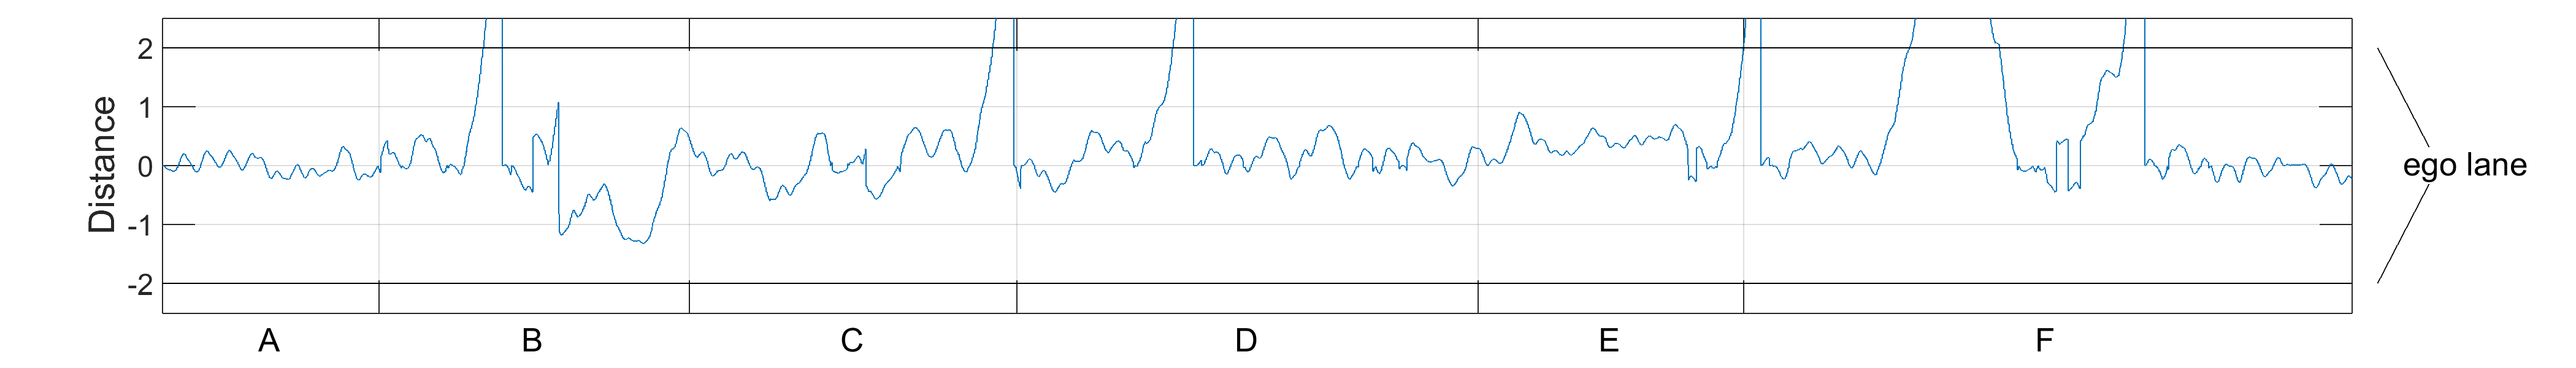
\includegraphics[scale=0.265]{../plots/dist_eval_log_distance_serpentine_06speed}
\vspace{0.5em}
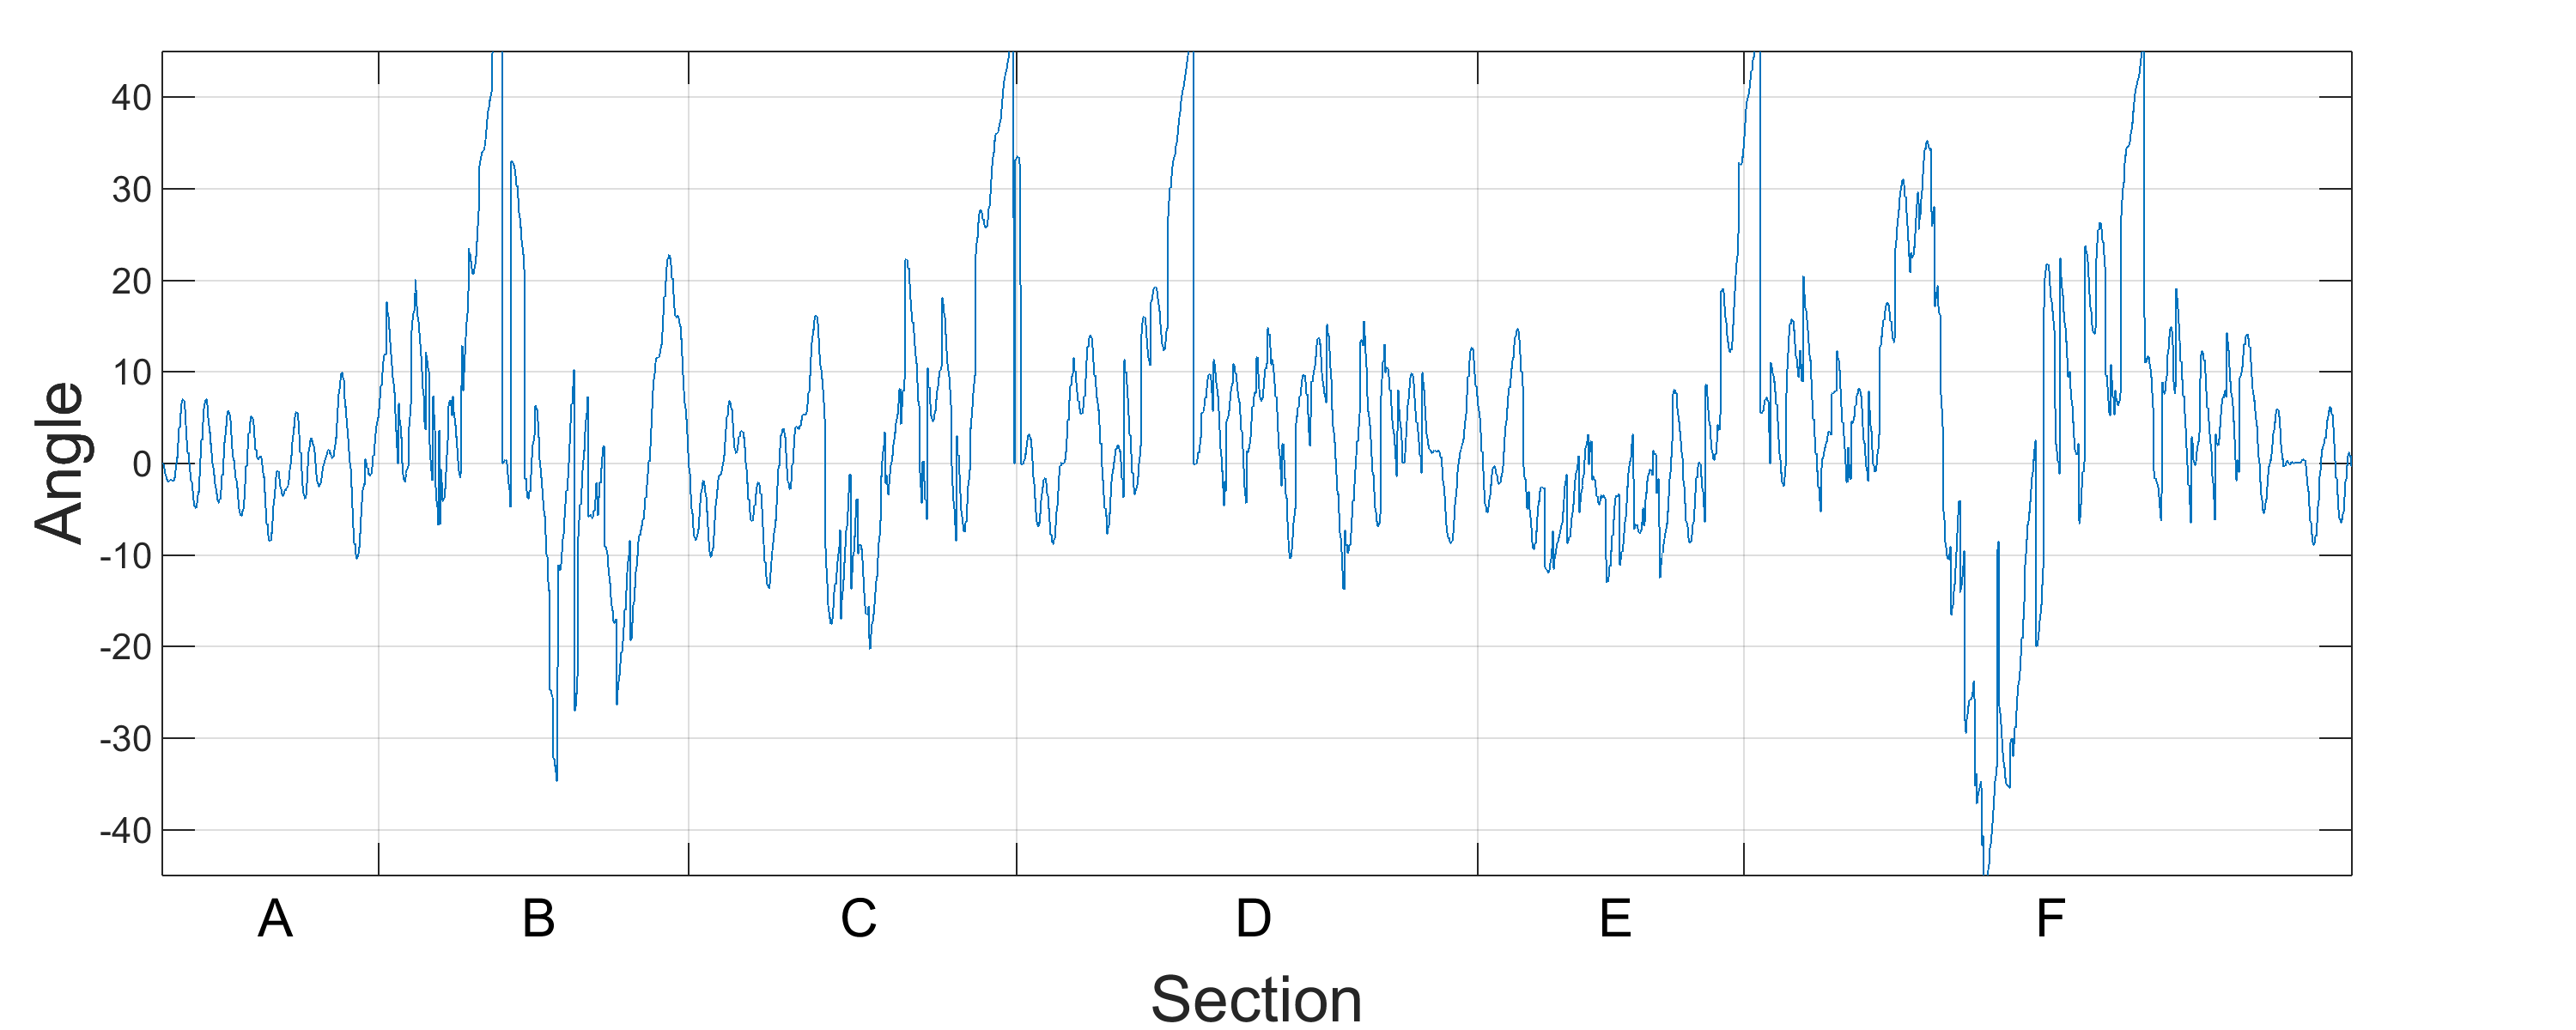
\includegraphics[scale=0.265]{../plots/ang_eval_log_distance_serpentine_06speed}
\vspace{-2.25em}
\caption{Distance-only approach. Distance in meters, angle in degrees.}
\label{distance06}
\vspace{1em}
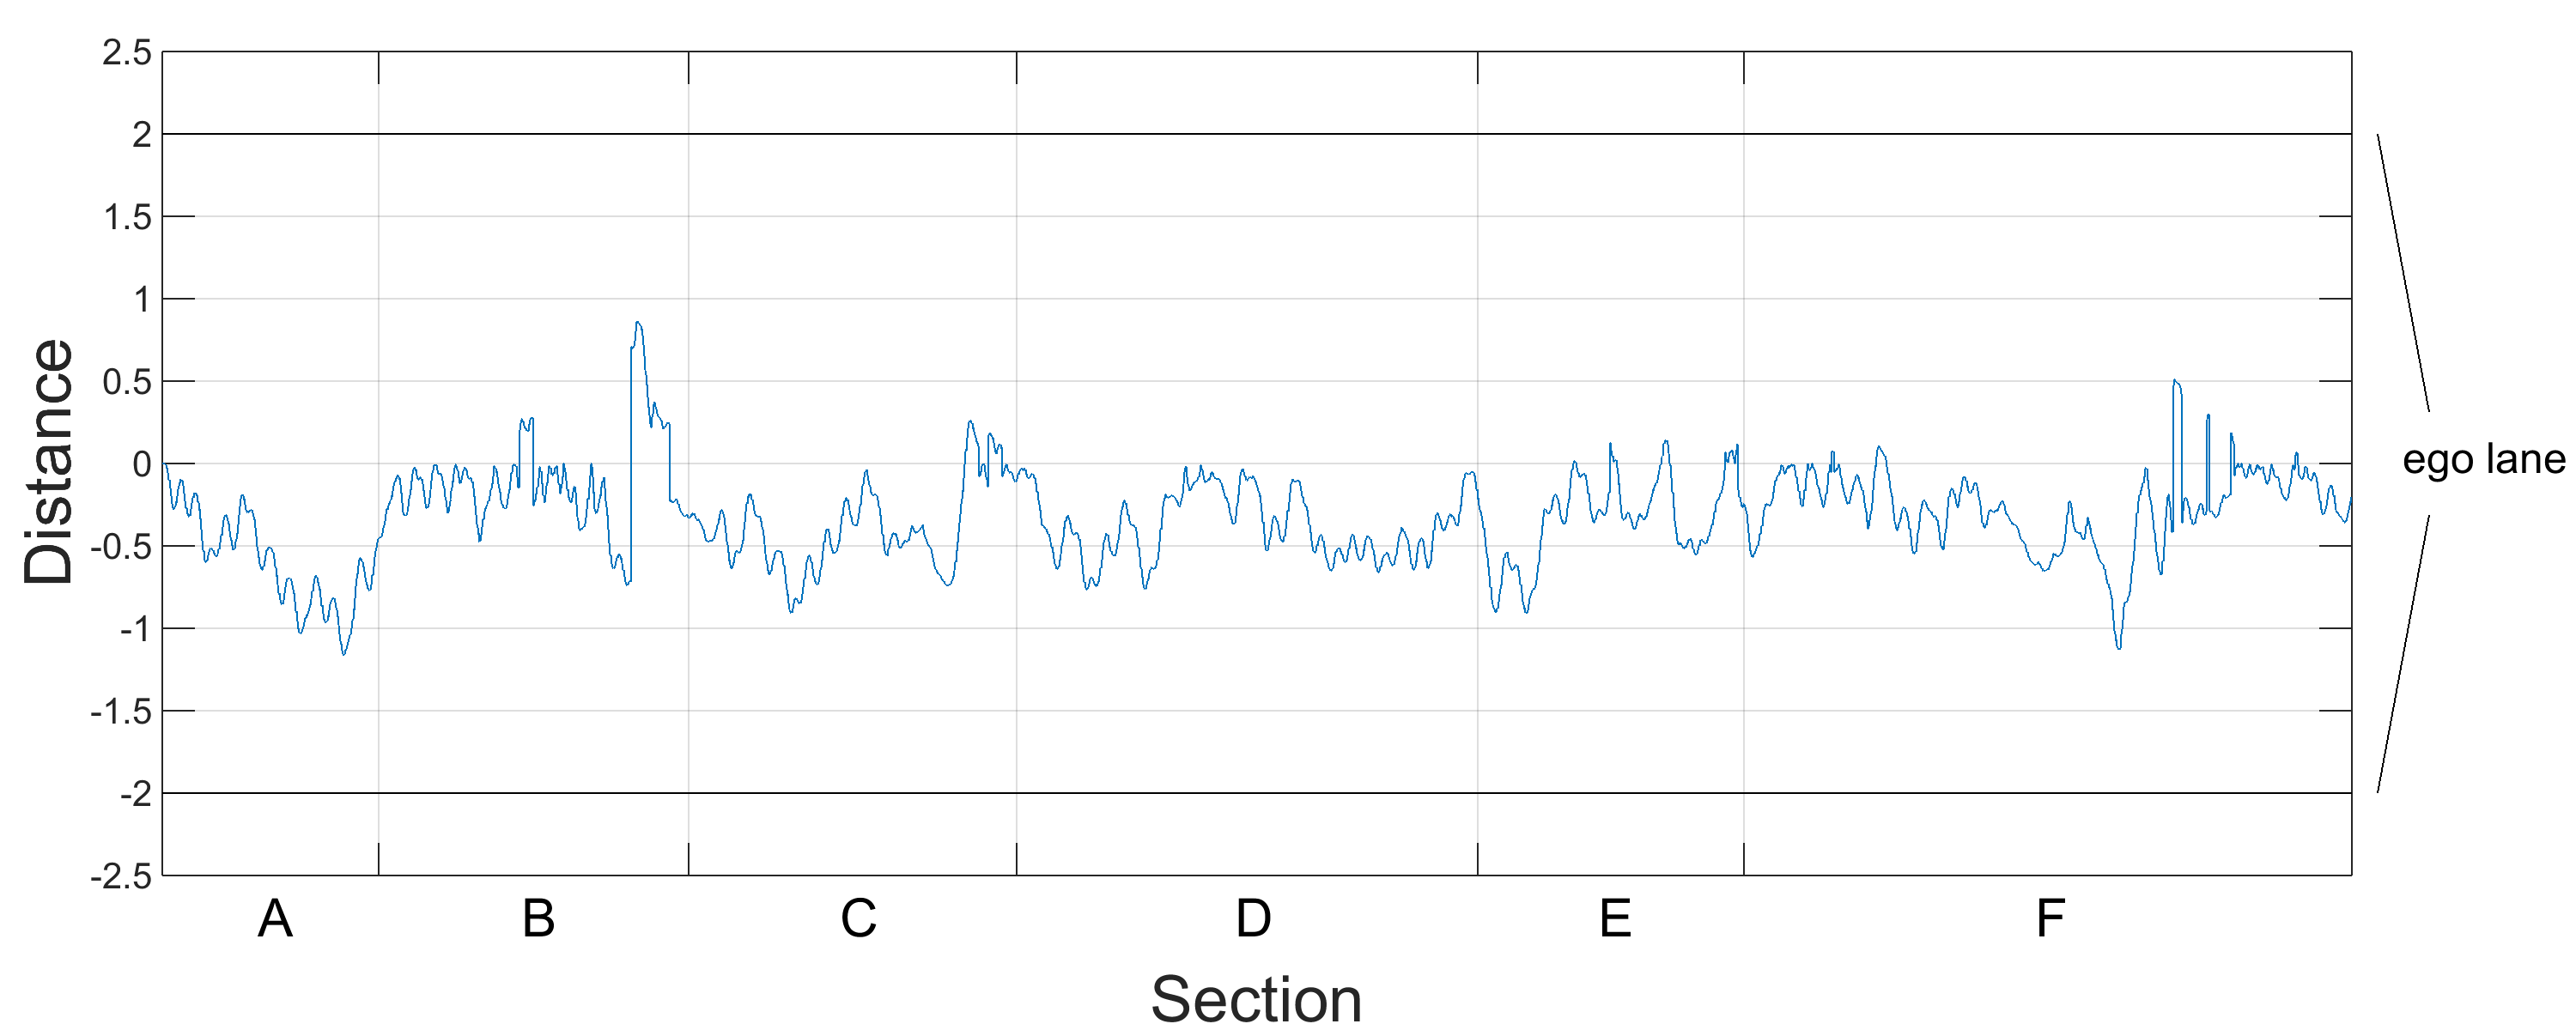
\includegraphics[scale=0.265]{../plots/dist_eval_log_dumb_actions_serpentine_06speed}
\vspace{0.5em}
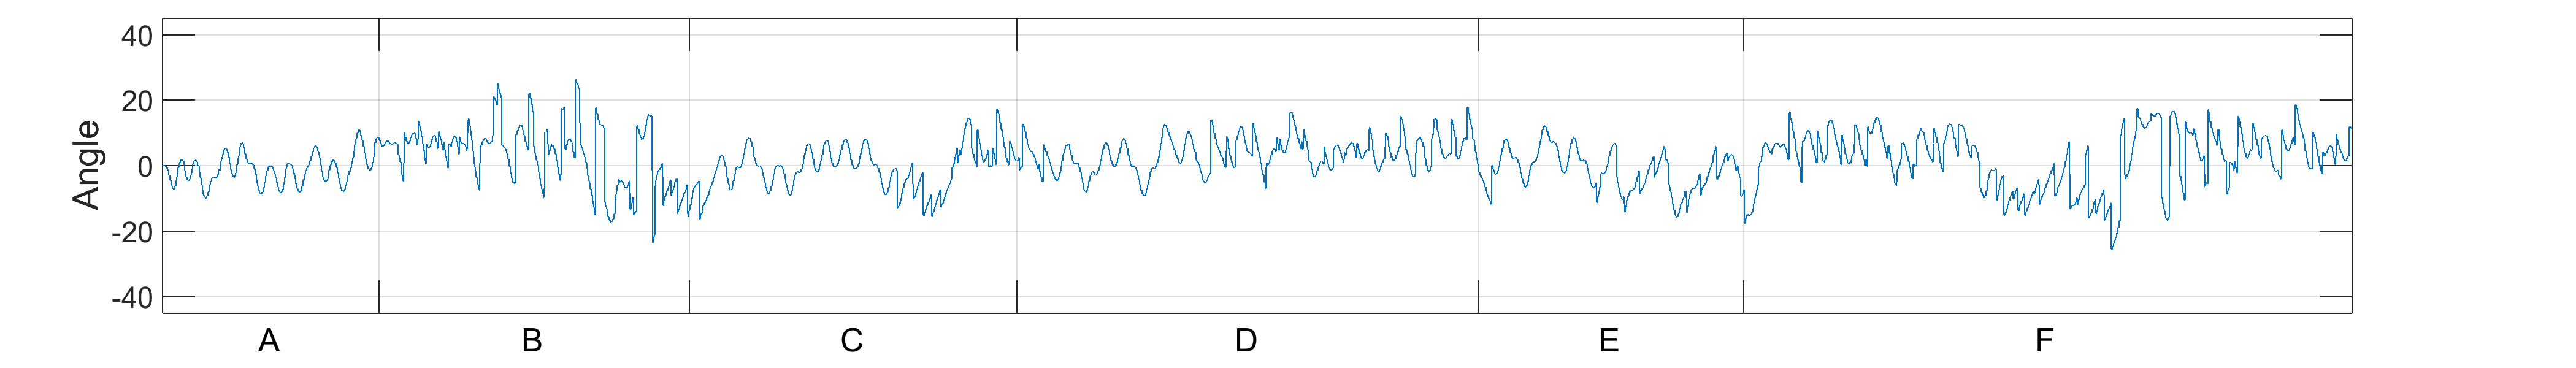
\includegraphics[scale=0.265]{../plots/ang_eval_log_dumb_actions_serpentine_06speed}
\vspace{-2.25em}\label{fig_first_case}
\caption{First action punishment added. Distance in meters, angle in degrees.}
\label{dumbactions06}
\end{figure*}

To evaluate each modification made to our reward function, we plotted distance and angle of the car in relation to the middle of the lane, as these are straightforward indicators for the quality of an approach. These plots were created for one lap on the same road, which was partitioned in several intervals for better comprehension of specific behaviour. For the distance plots we added lines indicating the designated lane to drive in. All plots are based on a trained vehicle for at least 6 million iterations, which means the training did already converge and would not change noticably if continued. 

Figure \ref{distance06} displays our first approach using nothing but a distance based reward. From the distance plot it becomes obvious that this approach was flawed. While the vehicle could handle straight sections like A and ones with wide curves as can be seen in the second half of D and most of E, it was not able to handle narrow curves at all. Whenever the car drove away too far from the road we had to reset it back on it's lane and continue from there. This is shown by the large spikes in the distance plot. One more interesting thing to note here is the wide, large spike in section F, where the car was not actually reset, but drove off the road at the end of the left turn, cut a corner and found back onto the road by chance. The fact that the car always drove off the road on the same side is mostly due to the fact that the longer narrow curves, which were more troublesome, consist almost entirely of left turns. The only such right turn would have been in F but was skipped by the car as we just explained. 
The angle plot fits this same picture. Whenever the car drove off the angle shows a large spike, because the car would leave a curve by driving straight or even turning in the wrong way. In section F we can again find our anomaly of the car cutting a corner, illustrated by the large negative spike.
Throughout the whole lap the distance and angle plot depict a very shaky behaviour, but it was obvious that the car understood it's task of staying in it's designated lane.

In section \ref{sec:approach} we explained our reasoning of adding an action based reward on top of the distance reward. The result of adding only the punishment for steering away from the road whilst already being located and turned away from it is displayed in figure \ref{dumbactions06}. The improvement over the distance-only based approach is immense. The vehicle was now able to finish the whole lap without leaving the road and being reset.

\begin{figure*}[!t]
\centering
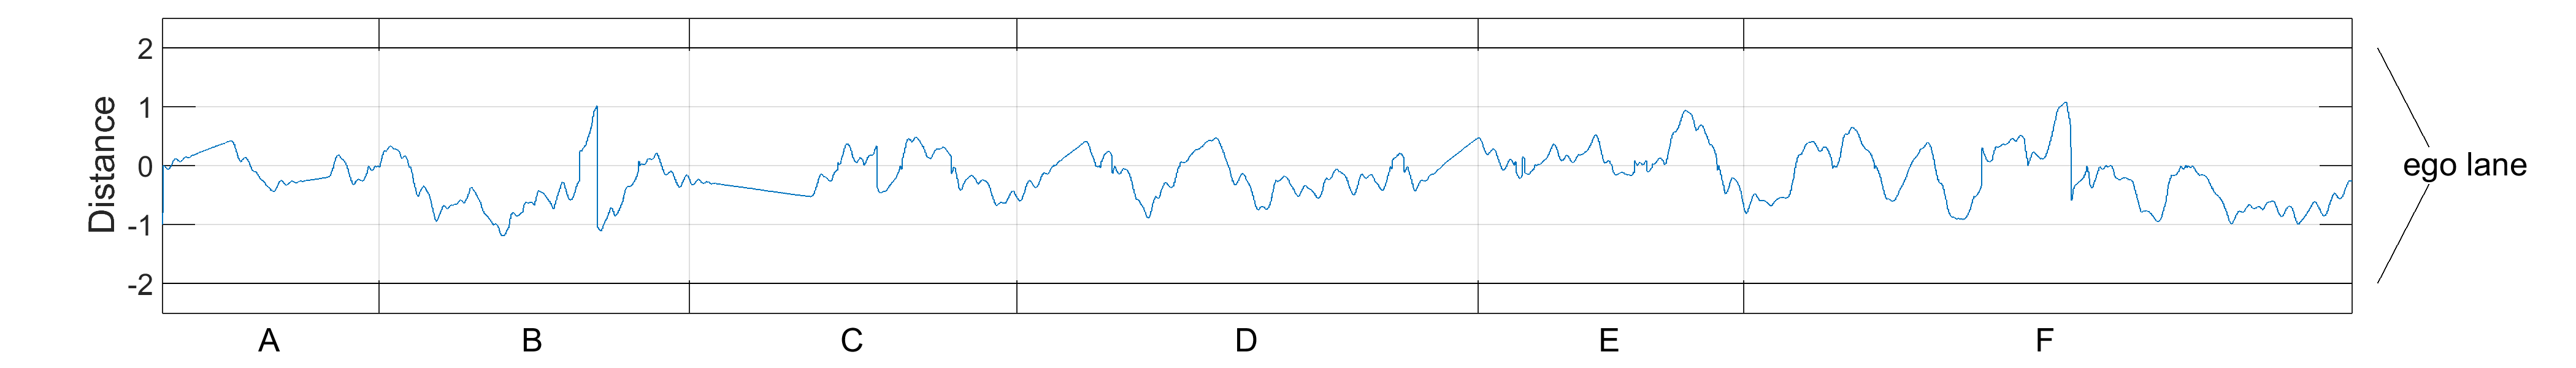
\includegraphics[scale=0.265]{../plots/dist_eval_log_straight_serpentine_06speed}
\vspace{0.5em}
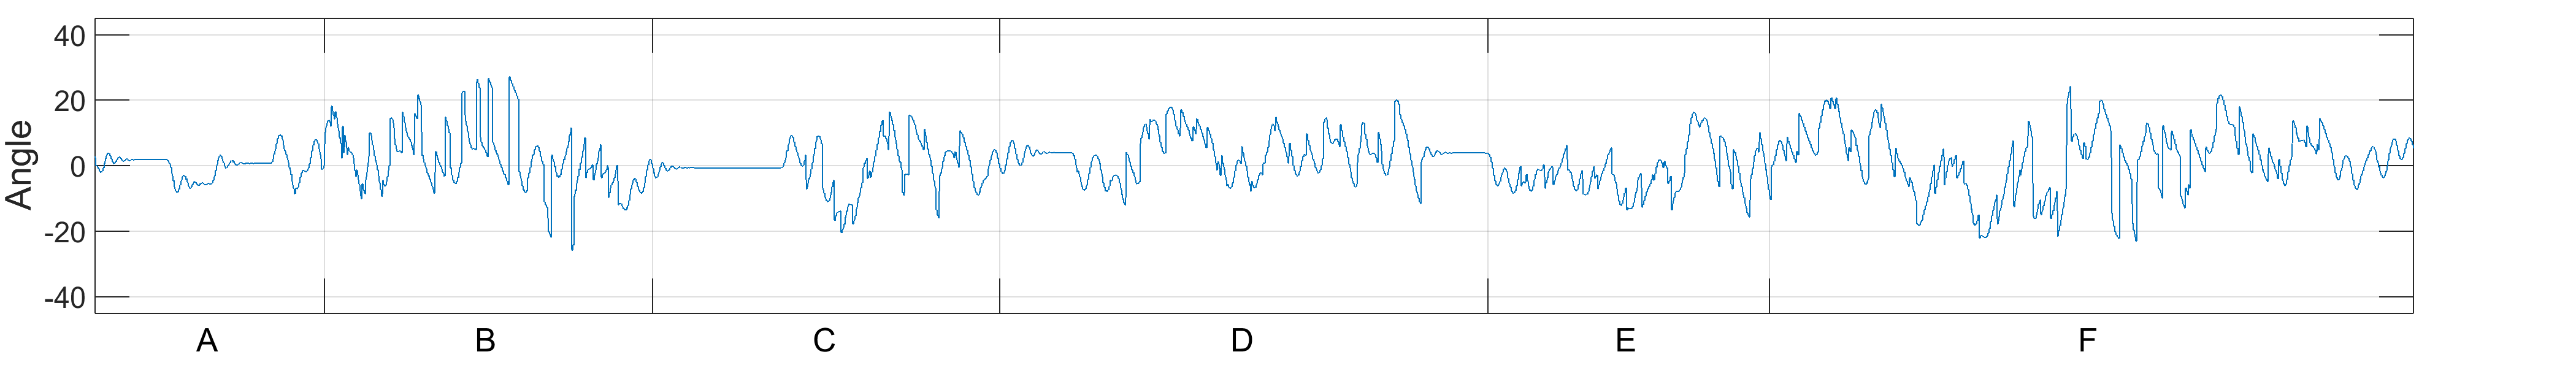
\includegraphics[scale=0.265]{../plots/ang_eval_log_straight_serpentine_06speed}
\vspace{-2.25em}
\caption{Straight action reward added. Distance in meters, angle in degrees.}
\label{distance06}
\vspace{1em}
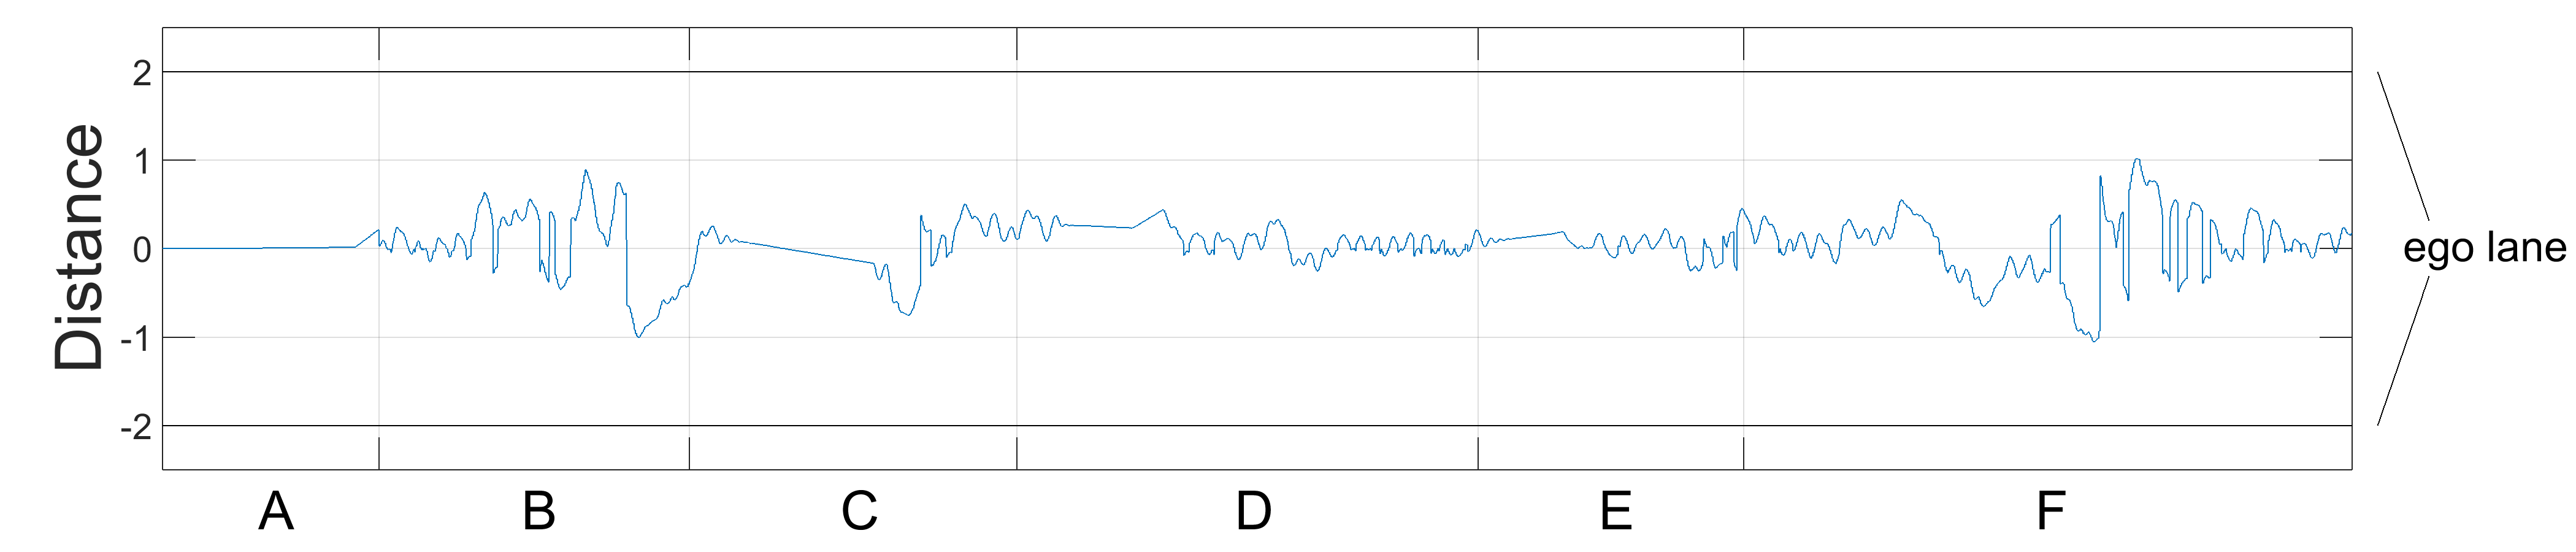
\includegraphics[scale=0.265]{../plots/dist_eval_log_smooth_serpentine_06speed}
\vspace{0.5em}
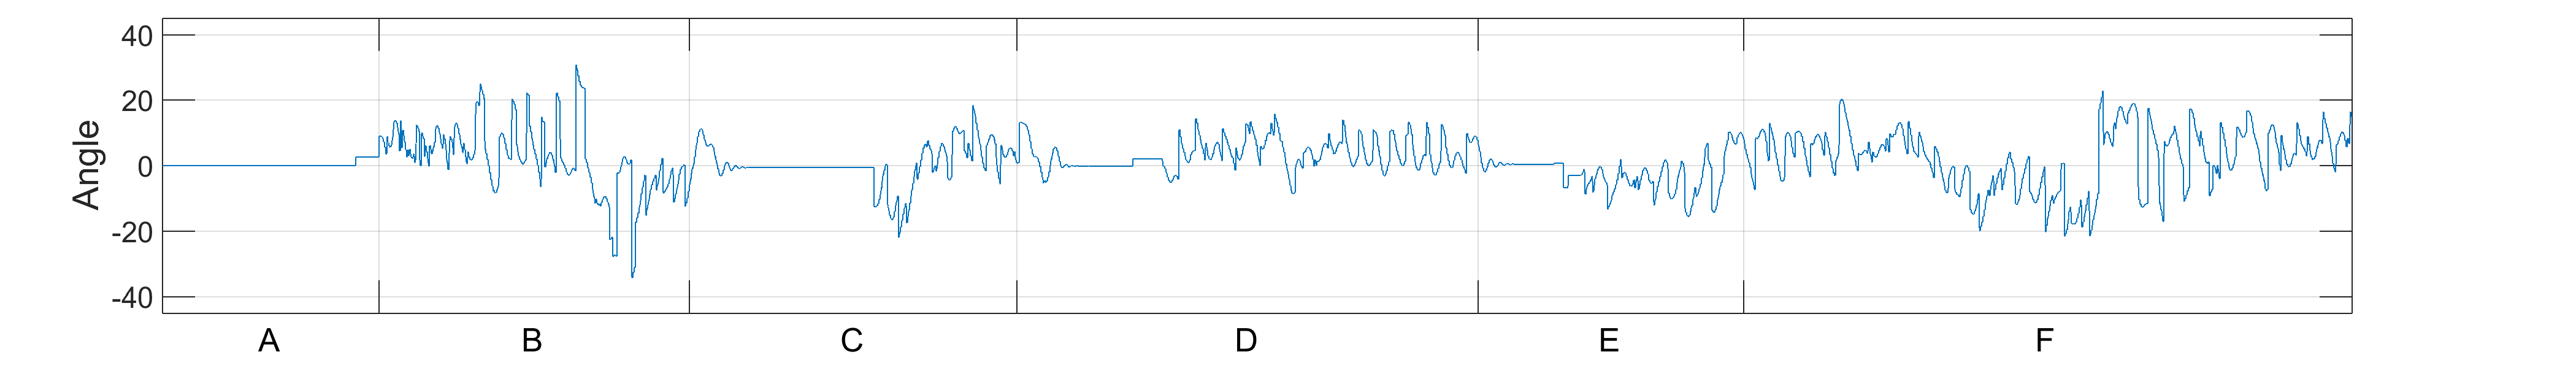
\includegraphics[scale=0.265]{../plots/ang_eval_log_smooth_serpentine_06speed}
\vspace{-2.25em}\label{fig_first_case}
\caption{Countersteering in curves punished. Distance in meters, angle in degrees.}
\label{dumbactions06}
\end{figure*}


%-RMSE plots for distance and angle?
%-for different track

